% Options for packages loaded elsewhere
\PassOptionsToPackage{unicode}{hyperref}
\PassOptionsToPackage{hyphens}{url}
\PassOptionsToPackage{dvipsnames,svgnames,x11names}{xcolor}
\documentclass[
  11pt]{article}
\usepackage{xcolor}
\usepackage[margin=1in]{geometry}
\usepackage{amsmath,amssymb}
\setcounter{secnumdepth}{-\maxdimen} % remove section numbering
\usepackage{iftex}
\ifPDFTeX
  \usepackage[T1]{fontenc}
  \usepackage[utf8]{inputenc}
  \usepackage{textcomp} % provide euro and other symbols
\else % if luatex or xetex
  \usepackage{unicode-math} % this also loads fontspec
  \defaultfontfeatures{Scale=MatchLowercase}
  \defaultfontfeatures[\rmfamily]{Ligatures=TeX,Scale=1}
\fi
\usepackage{lmodern}
\ifPDFTeX\else
  % xetex/luatex font selection
\fi
% Use upquote if available, for straight quotes in verbatim environments
\IfFileExists{upquote.sty}{\usepackage{upquote}}{}
\IfFileExists{microtype.sty}{% use microtype if available
  \usepackage[]{microtype}
  \UseMicrotypeSet[protrusion]{basicmath} % disable protrusion for tt fonts
}{}
\makeatletter
\@ifundefined{KOMAClassName}{% if non-KOMA class
  \IfFileExists{parskip.sty}{%
    \usepackage{parskip}
  }{% else
    \setlength{\parindent}{0pt}
    \setlength{\parskip}{6pt plus 2pt minus 1pt}}
}{% if KOMA class
  \KOMAoptions{parskip=half}}
\makeatother
\usepackage{color}
\usepackage{fancyvrb}
\newcommand{\VerbBar}{|}
\newcommand{\VERB}{\Verb[commandchars=\\\{\}]}
\DefineVerbatimEnvironment{Highlighting}{Verbatim}{commandchars=\\\{\}}
% Add ',fontsize=\small' for more characters per line
\newenvironment{Shaded}{}{}
\newcommand{\AlertTok}[1]{\textcolor[rgb]{1.00,0.00,0.00}{\textbf{#1}}}
\newcommand{\AnnotationTok}[1]{\textcolor[rgb]{0.38,0.63,0.69}{\textbf{\textit{#1}}}}
\newcommand{\AttributeTok}[1]{\textcolor[rgb]{0.49,0.56,0.16}{#1}}
\newcommand{\BaseNTok}[1]{\textcolor[rgb]{0.25,0.63,0.44}{#1}}
\newcommand{\BuiltInTok}[1]{\textcolor[rgb]{0.00,0.50,0.00}{#1}}
\newcommand{\CharTok}[1]{\textcolor[rgb]{0.25,0.44,0.63}{#1}}
\newcommand{\CommentTok}[1]{\textcolor[rgb]{0.38,0.63,0.69}{\textit{#1}}}
\newcommand{\CommentVarTok}[1]{\textcolor[rgb]{0.38,0.63,0.69}{\textbf{\textit{#1}}}}
\newcommand{\ConstantTok}[1]{\textcolor[rgb]{0.53,0.00,0.00}{#1}}
\newcommand{\ControlFlowTok}[1]{\textcolor[rgb]{0.00,0.44,0.13}{\textbf{#1}}}
\newcommand{\DataTypeTok}[1]{\textcolor[rgb]{0.56,0.13,0.00}{#1}}
\newcommand{\DecValTok}[1]{\textcolor[rgb]{0.25,0.63,0.44}{#1}}
\newcommand{\DocumentationTok}[1]{\textcolor[rgb]{0.73,0.13,0.13}{\textit{#1}}}
\newcommand{\ErrorTok}[1]{\textcolor[rgb]{1.00,0.00,0.00}{\textbf{#1}}}
\newcommand{\ExtensionTok}[1]{#1}
\newcommand{\FloatTok}[1]{\textcolor[rgb]{0.25,0.63,0.44}{#1}}
\newcommand{\FunctionTok}[1]{\textcolor[rgb]{0.02,0.16,0.49}{#1}}
\newcommand{\ImportTok}[1]{\textcolor[rgb]{0.00,0.50,0.00}{\textbf{#1}}}
\newcommand{\InformationTok}[1]{\textcolor[rgb]{0.38,0.63,0.69}{\textbf{\textit{#1}}}}
\newcommand{\KeywordTok}[1]{\textcolor[rgb]{0.00,0.44,0.13}{\textbf{#1}}}
\newcommand{\NormalTok}[1]{#1}
\newcommand{\OperatorTok}[1]{\textcolor[rgb]{0.40,0.40,0.40}{#1}}
\newcommand{\OtherTok}[1]{\textcolor[rgb]{0.00,0.44,0.13}{#1}}
\newcommand{\PreprocessorTok}[1]{\textcolor[rgb]{0.74,0.48,0.00}{#1}}
\newcommand{\RegionMarkerTok}[1]{#1}
\newcommand{\SpecialCharTok}[1]{\textcolor[rgb]{0.25,0.44,0.63}{#1}}
\newcommand{\SpecialStringTok}[1]{\textcolor[rgb]{0.73,0.40,0.53}{#1}}
\newcommand{\StringTok}[1]{\textcolor[rgb]{0.25,0.44,0.63}{#1}}
\newcommand{\VariableTok}[1]{\textcolor[rgb]{0.10,0.09,0.49}{#1}}
\newcommand{\VerbatimStringTok}[1]{\textcolor[rgb]{0.25,0.44,0.63}{#1}}
\newcommand{\WarningTok}[1]{\textcolor[rgb]{0.38,0.63,0.69}{\textbf{\textit{#1}}}}
\usepackage{longtable,booktabs,array}
\newcounter{none} % for unnumbered tables
\usepackage{calc} % for calculating minipage widths
% Correct order of tables after \paragraph or \subparagraph
\usepackage{etoolbox}
\makeatletter
\patchcmd\longtable{\par}{\if@noskipsec\mbox{}\fi\par}{}{}
\makeatother
% Allow footnotes in longtable head/foot
\IfFileExists{footnotehyper.sty}{\usepackage{footnotehyper}}{\usepackage{footnote}}
\makesavenoteenv{longtable}
\usepackage{graphicx}
\makeatletter
\newsavebox\pandoc@box
\newcommand*\pandocbounded[1]{% scales image to fit in text height/width
  \sbox\pandoc@box{#1}%
  \Gscale@div\@tempa{\textheight}{\dimexpr\ht\pandoc@box+\dp\pandoc@box\relax}%
  \Gscale@div\@tempb{\linewidth}{\wd\pandoc@box}%
  \ifdim\@tempb\p@<\@tempa\p@\let\@tempa\@tempb\fi% select the smaller of both
  \ifdim\@tempa\p@<\p@\scalebox{\@tempa}{\usebox\pandoc@box}%
  \else\usebox{\pandoc@box}%
  \fi%
}
% Set default figure placement to htbp
\def\fps@figure{htbp}
\makeatother
\setlength{\emergencystretch}{3em} % prevent overfull lines
\providecommand{\tightlist}{%
  \setlength{\itemsep}{0pt}\setlength{\parskip}{0pt}}
% Preamble for the Sentinela manuscript (xelatex).
% Injected into the pandoc-generated standalone LaTeX via --include-in-header.
% Gives the paper a clean single-column academic look with good typography,
% booktabs tables, sensible figure defaults, and coloured hyperlinks.

% --- fonts (xelatex) ---
\usepackage{fontspec}
\IfFontExistsTF{TeX Gyre Pagella}{\setmainfont{TeX Gyre Pagella}}{}
\IfFontExistsTF{TeX Gyre Heros}{\setsansfont{TeX Gyre Heros}}{}
\IfFontExistsTF{TeX Gyre Cursor}{\setmonofont{TeX Gyre Cursor}}{}
\usepackage{microtype}

% --- maths glyph coverage (so >=, <=, approx render in text) ---
\usepackage{newunicodechar}
\newunicodechar{≥}{\ensuremath{\geq}}
\newunicodechar{≤}{\ensuremath{\leq}}
\newunicodechar{≈}{\ensuremath{\approx}}
\newunicodechar{α}{\ensuremath{\alpha}}
\newunicodechar{σ}{\ensuremath{\sigma}}
\newunicodechar{×}{\ensuremath{\times}}
\newunicodechar{→}{\ensuremath{\rightarrow}}
\newunicodechar{²}{\ensuremath{^{2}}}
\newunicodechar{³}{\ensuremath{^{3}}}
\newunicodechar{∝}{\ensuremath{\propto}}

% --- tables / figures ---
\usepackage{booktabs}
\usepackage{longtable}
\usepackage{graphicx}
\usepackage{float}
\usepackage[font=small,labelfont=bf,skip=4pt]{caption}
\setkeys{Gin}{width=\linewidth,keepaspectratio}

% --- section styling ---
% Headers use the same serif body font (bold) so the paper is typographically
% consistent throughout — no sans/serif split.
\usepackage{titlesec}
\titleformat{\section}{\large\bfseries}{\thesection}{0.6em}{}
\titleformat{\subsection}{\normalsize\bfseries}{\thesubsection}{0.6em}{}
\titlespacing*{\section}{0pt}{1.4ex plus 1ex minus .2ex}{0.8ex plus .2ex}

% --- abstract a touch narrower for a journal feel ---
\usepackage{changepage}

% --- header / footer ---
\usepackage{fancyhdr}
\pagestyle{fancy}
\fancyhf{}
\fancyhead[L]{\footnotesize Sentinela}
\fancyhead[R]{\footnotesize Forecasting Brazil's Next Tailings-Dam Disaster}
\fancyfoot[C]{\thepage}
\renewcommand{\headrulewidth}{0.3pt}

% Tighten list spacing.
\usepackage{enumitem}
\setlist{itemsep=2pt, topsep=3pt}
\usepackage{bookmark}
\IfFileExists{xurl.sty}{\usepackage{xurl}}{} % add URL line breaks if available
\urlstyle{same}
\hypersetup{
  pdftitle={Forecasting Brazil's Next Tailings-Dam Disaster},
  colorlinks=true,
  linkcolor={RoyalBlue},
  filecolor={Maroon},
  citecolor={Blue},
  urlcolor={RoyalBlue},
  pdfcreator={LaTeX via pandoc}}

\author{}
\date{}

\begin{document}

% Custom title page, injected via pandoc --include-before-body.
% The graphics path is relative to paper/ (where xelatex compiles); the
% Overleaf bundle script rewrites ../figures/ -> figures/.
\begin{titlepage}
\centering
\vspace*{1.0cm}

{\bfseries\fontsize{30}{36}\selectfont
Forecasting Brazil's\\[2pt] Next Tailings-Dam Disaster\par}

\vspace{0.7cm}
{\large\itshape Sentinela --- a calibrated hierarchical-Bayesian forecaster\\
for Brazilian mine-tailings dam failures\par}

\vspace{0.5cm}
{\color{RoyalBlue}\rule{0.82\linewidth}{1.2pt}\par}

\vspace{0.9cm}
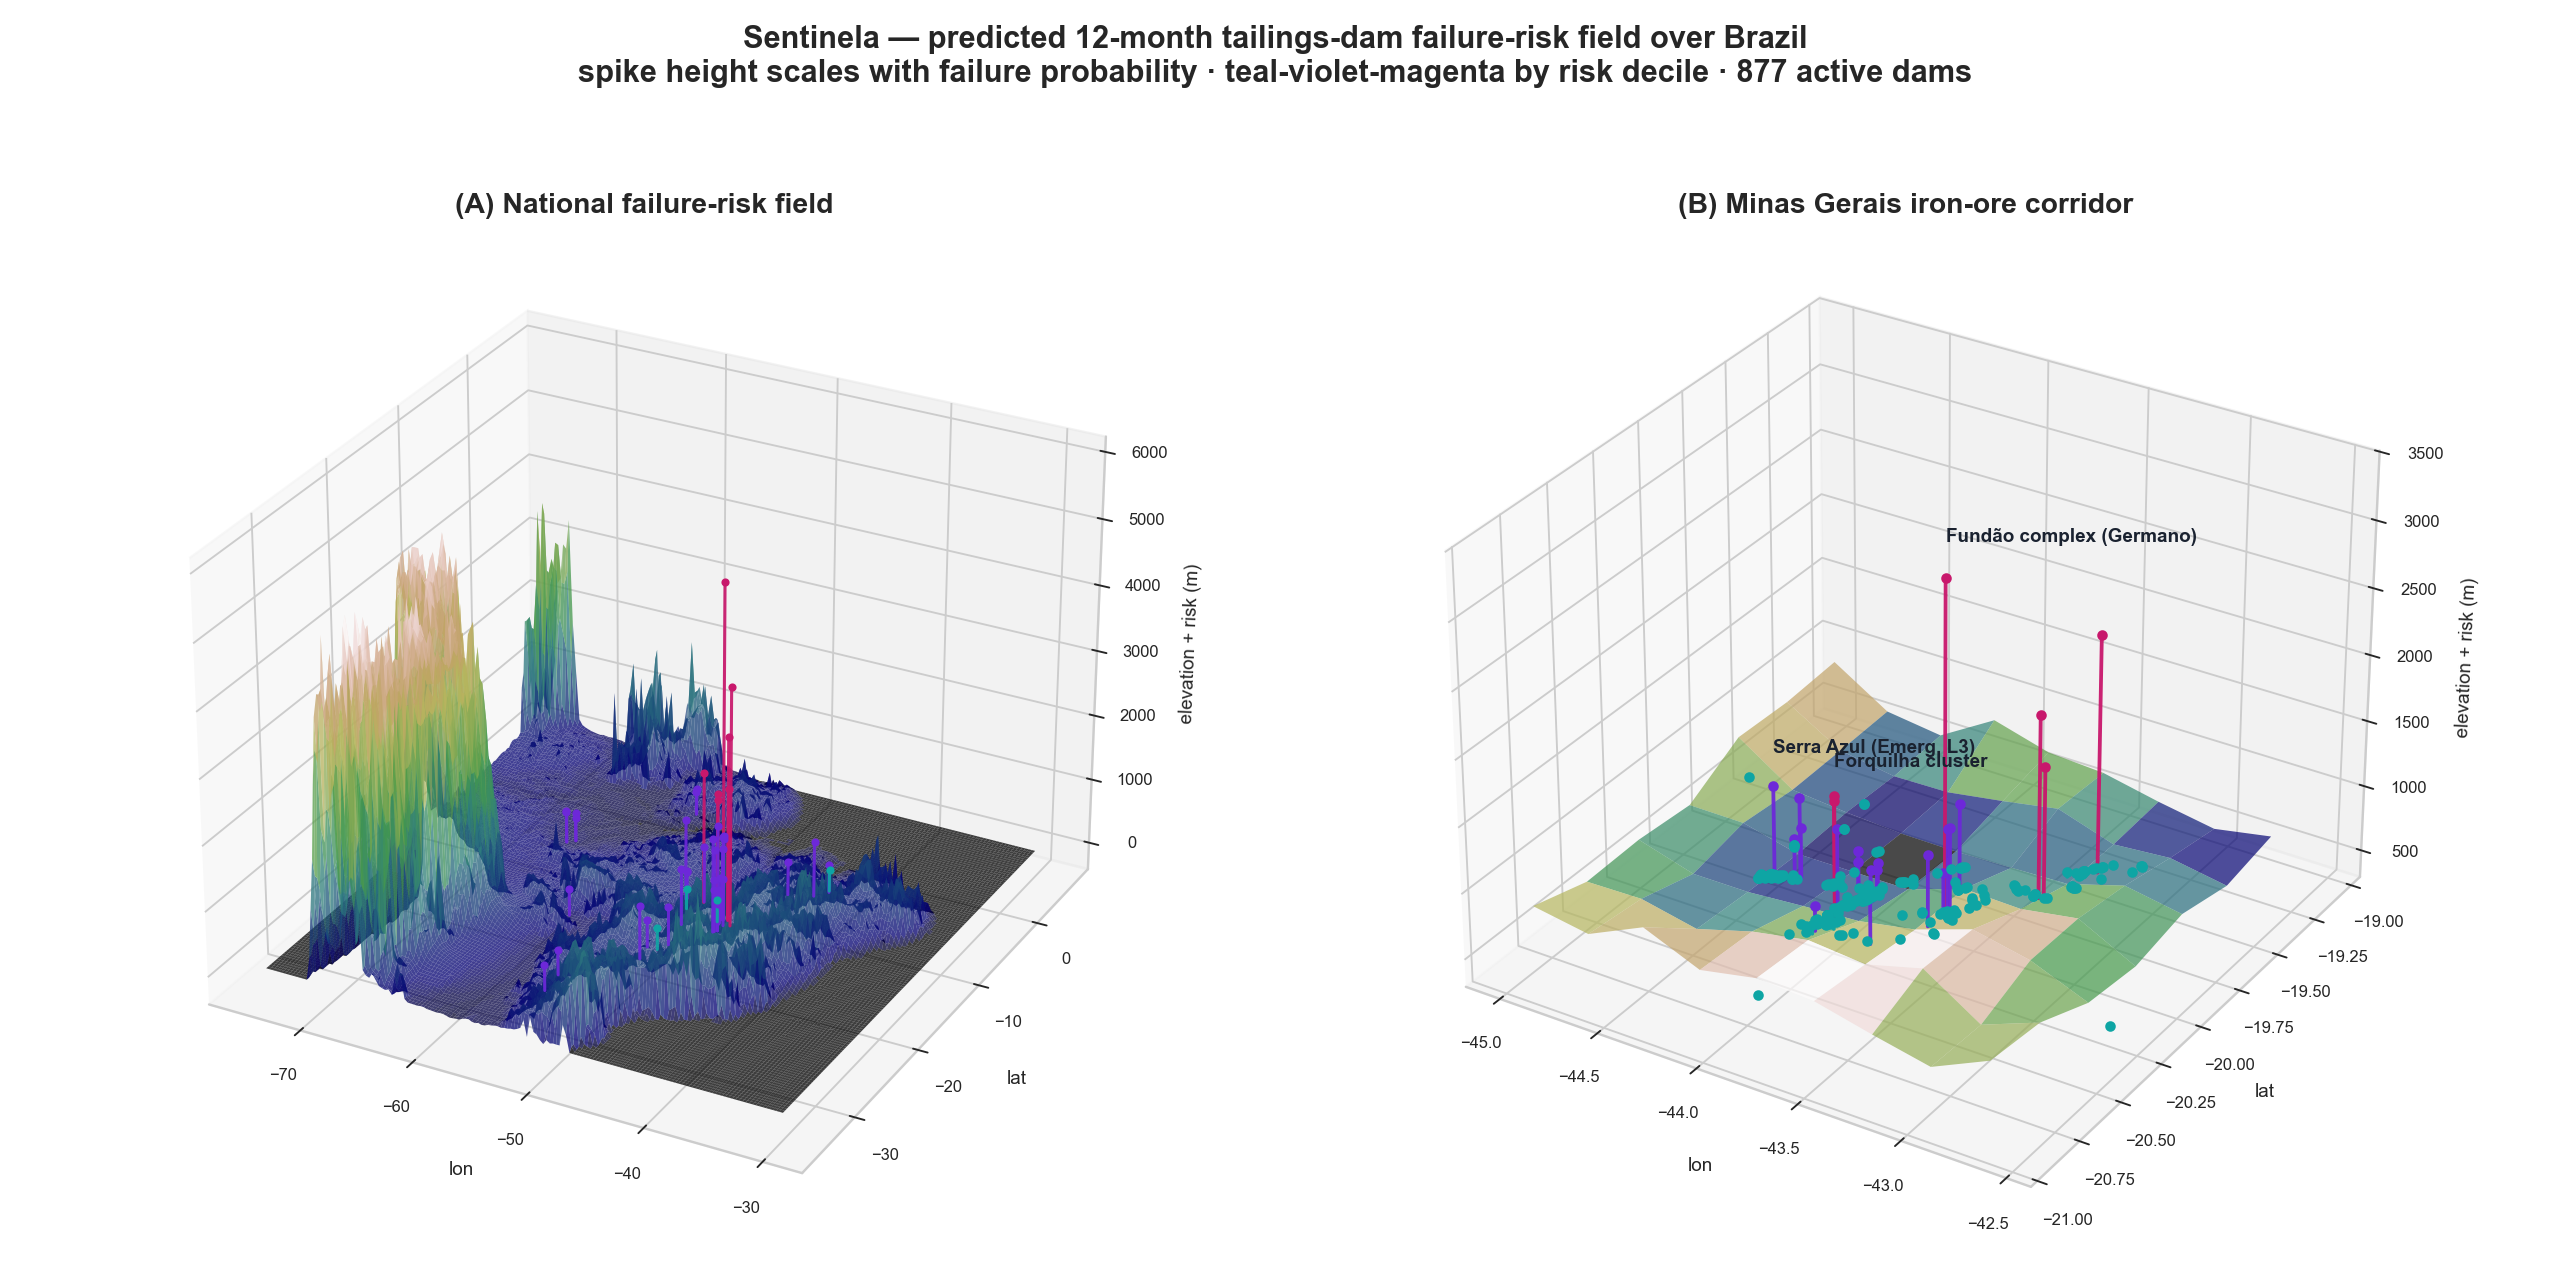
\includegraphics[width=\linewidth]{../figures/fig0_hero.png}

\vspace{0.5cm}
{\footnotesize\itshape Predicted 12-month failure-risk field over Brazil's terrain.
(A) national view; (B) Minas Gerais iron-ore corridor with the reference-failure
complexes labelled. Spike height scales with failure probability; colour runs
teal $\rightarrow$ violet $\rightarrow$ magenta by risk decile.\par}

\vfill

{\large\bfseries Viktor Smirnov\par}
{\normalsize Arakon\par}
\vspace{0.3cm}
{\normalsize 24 May 2026 \quad\textbullet\quad pre-print\par}

\vspace{0.6cm}
{\footnotesize\color{Gray}
Open data \textbullet\ open code \textbullet\ reproducible from a clean clone\\
\texttt{github.com/ViktorSmirnov71/sentinela-bayes-br}\par}

\end{titlepage}

{
\setcounter{tocdepth}{2}
\tableofcontents
}
\section{Abstract}\label{abstract}

Catastrophic failure of mine-tailings storage facilities (TSFs) in
Brazil killed at least 289 people in two events in the last decade
(Mariana 2015, Brumadinho 2019). After Brumadinho, three things became
reproducibly true: the Brazilian regulator publishes a national TSF
registry (SIGBM, 911 dams in our 2026 snapshot); the European Copernicus
programme freely distributes Sentinel-1 SAR with a 6--12 day revisit
over all of Brazil since 2014; and post-mortem analyses (Grebby et
al.~2021; Carlà et al.~2019) confirmed that the B1 Córrego do Feijão
collapse was detectable from Sentinel-1 InSAR at least five months in
advance. Yet there is no published, openly reproducible, per-dam
probabilistic forecaster that uses these inputs.

We present \textbf{Sentinela}, a hierarchical-Bayesian model that
produces a calibrated 12-month-ahead failure probability for every
active Brazilian mine-tailings dam from purely public data. The model
composes a literature-informed Beta-Binomial construction-method
posterior, a James--Stein-shrunk per-operator random effect, bounded
logit shifts for engineering features (height, volume, age, regulator
risk category), and a bounded InSAR-precursor term derived from
Sentinel-1 line-of-sight displacement. We report three results. (1) On
the 2026 SIGBM snapshot the engineering-feature ranking independently
surfaces the dams ANM has separately placed under emergency
declarations: the single Emergency-Level-3 dam in the country (Barragem
Serra Azul) and the entire Level-2 Forquilha cluster appear in the
top-15, despite the model receiving no emergency-level input --- an
external validation that the within-construction-class ordering is
meaningful. (2) We process 148 Sentinel-1 interferograms through ASF
HyP3 at the actual coordinates of both reference failures and run a
month-by-month retrospective; at Brumadinho B1 the predicted risk spikes
in April 2018, inside the ``definitive but emergent risk'' window
reported independently by Grebby et al.~(2021), a partial replication of
the published precursor with a purely open pipeline. (3) We document a
``registry-amnesia'' bias (failed dams are struck from SIGBM
post-failure) and a cross-relative-orbit SBAS pairing failure mode (100
\% of our HyP3 failures), both of which are methodologically instructive
at population scale. We argue that in the one-linked-positive regime
that characterises this problem, a transparent literature-prior Bayesian
model is the honest choice over discriminative learners, which we show
empirically either memorise the single positive or collapse to zero. All
code, data, figures, the 3D visualisation, and this manuscript are
openly released and reproducible from a clean clone in five commands.

\section{1. Introduction}\label{introduction}

A tailings dam is the engineered wall that retains the slurry by-product
of mineral extraction. Catastrophic failure releases the impounded
volume as a flowing mudwave. Mariana 2015 destroyed Bento Rodrigues and
contaminated 600 km of the Doce river. Brumadinho 2019 killed
approximately 270 people in 90 seconds. These are not isolated events:
the World Mine Tailings Failures catalogue records eight Brazilian
severity-4-or-higher events since 1986.

Three developments after Brumadinho make per-dam quantitative
forecasting newly tractable:

\begin{enumerate}
\def\labelenumi{\arabic{enumi}.}
\tightlist
\item
  \textbf{SIGBM} (Sistema Integrado de Gestão de Barragens de Mineração)
  --- the Agência Nacional de Mineração's national TSF registry, public
  since 2019 {[}@anm\_sigbm{]}.
\item
  \textbf{Sentinel-1} --- ESA Copernicus C-band SAR, full archive open
  since 2014, 6--12-day revisit, millimetre-precision interferometric
  ground-deformation measurement.
\item
  \textbf{Post-mortem replication studies} {[}@grebby2021; @carla2019;
  @du2020; @gama2023{]} that confirm the B1 collapse left a clear InSAR
  signature months before failure.
\end{enumerate}

The literature has progressed from \emph{``InSAR can post-hoc identify
precursors at known failures''} to \emph{``InSAR + ML can flag elevated
risk at active facilities''}. No published model jointly (a) uses SIGBM
as the cohort, (b) propagates calibrated uncertainty, and (c) is
reproducibly open from data to forecast. This paper fills that gap with
the simplest methodology that does so.

\section{2. Related work}\label{related-work}

\subsection{2.1 Single-event precursor
reconstruction}\label{single-event-precursor-reconstruction}

@grebby2021 applied advanced InSAR analysis to Sentinel-1 over B1 and
detected ground-deformation precursors ≥5 months before the 25 January
2019 collapse. @carla2019 independently derived an inverse-velocity
time-of-failure prediction. @du2020 performed an InSAR time-series risk
assessment of the Brumadinho cluster. @gama2023 published a slip-surface
mechanism account attributing the failure to delayed static
liquefaction. @mura2018 used DInSAR with TerraSAR-X to monitor the
surviving dikes at the Germano complex post-Fundão. These works
establish that the geophysical precursor signal exists in
publicly-available Sentinel-1 data at known failures.

\subsection{2.2 Generalised early-warning and ML on
InSAR}\label{generalised-early-warning-and-ml-on-insar}

@macchiarulo2023 reduced false alarms by combining InSAR deformation
with SAR-derived moisture content. @manconi2024 catalogued practical
considerations for operational Sentinel-1 monitoring of tailings dams.
@zhang2025 proposed an InSAR framework that robustly separates
consolidation settlement from failure-relevant deformation. @zheng2025
integrated InSAR with 3D numerical models. None of these output
calibrated per-dam probabilities at population scale, none jointly use
construction-type metadata, and none are reproducibly open from data to
forecast.

\subsection{2.3 Population-scale risk
classification}\label{population-scale-risk-classification}

@delima2022 classified Brazilian TSFs by risk using SIGBM-derived
features (without InSAR), but treats ANM's administrative risk score as
the target, not failure events. @rana2021 published a global statistical
model of tailings-dam failure frequency vs.~construction type using WMTF
data --- a population baseline rate, not a per-dam forecast.

\subsection{2.4 The gap}\label{the-gap}

Combining the three lines: - Post-hoc precursor work shows the
\emph{signal exists}. - Methodological InSAR-ML work shows the
\emph{signal can be extracted}. - Population-scale work establishes a
\emph{cohort} but uses administrative scores as labels.

What does not exist: a reproducible per-dam probabilistic forecaster for
Brazilian TSFs that (i) uses SIGBM as its cohort, (ii) ingests
Sentinel-1 InSAR-derived precursor features, (iii) is trained against
documented failure or near-miss events with explicit survival censoring,
and (iv) is evaluated with proper uncertainty quantification. This is
the target of Sentinela.

\section{3. Data}\label{data}

We assemble the analysis from five categories of public open data; full
provenance, schema, and access mechanisms are documented in
\texttt{docs/03-data.md} and \texttt{data/README.md} of the open-source
repository.

\subsection{3.1 Cohort: SIGBM}\label{cohort-sigbm}

The Agência Nacional de Mineração's public web app at
\texttt{app.anm.gov.br/sigbm/publico} provides a manual CSV export with
911 dams (2026-05-21 snapshot). Schema includes construction method
(upstream / downstream / centerline / single-stage / dyke / unknown),
current height and volume, primary ore, operator CNPJ, the ANM Risk
Category (CRI) and Damage-Potential Category (DPA), declared emergency
level, and operational status. The export is semicolon-delimited
UTF-8-with-BOM with Brazilian decimal format and DMS coordinates; we
canonicalise these in \texttt{src/sentinela/io/sigbm.py}.

\textbf{Snapshot composition.} The cohort spans 21 states, dominated by
Minas Gerais (35\%), Mato Grosso (20\%), and Pará (13\%). Construction
methods are distributed 53\% single-stage, 24\% downstream, 13\%
centerline, 5\% upstream (the historically dangerous class with 45
dams), 5\% unknown. As of the snapshot, 822 dams are at no declared
emergency level, 12 at Alert level, 69 at Emergency Level 1, 7 at
Emergency Level 2, and 1 at Emergency Level 3 --- the single
most-immediately-concerning structure currently in Brazil.

\textbf{Methodology note --- registry amnesia.} ANM removes failed dams
from the active SIGBM registry post-failure. Vale's B1 Córrego do Feijão
(2019), Samarco's Fundão (2015), and Herculano's B1 (2014) are all
absent from the current export. The Fundão event has a credible proxy
via dam\_id 8765, \emph{Barragem de Germano} --- the surviving Samarco
structure at the same mining complex, now in decommissioning. Other
historical failures need pre-failure SIGBM snapshots (obtainable from
Wayback Machine archives or by FOI request) to be modelled
prospectively. This biases the cohort toward ``dams that have not yet
failed'' and is the single biggest limitation of the present work.

\subsection{3.2 Labels: Brazilian failure
events}\label{labels-brazilian-failure-events}

A hand-curated, citation-anchored table of eight documented Brazilian
TSF-failure events from 1986 to 2022 is committed to the repository at
\texttt{data/external/brazilian\_failures.csv}. The table preserves the
Bowker--Chambers severity coding {[}@wmtf{]}; the primary cutoff for the
positive class is severity ≥ 4.

\subsection{3.3 Precursor signal: Sentinel-1
InSAR}\label{precursor-signal-sentinel-1-insar}

Sentinel-1 SLC scenes intersecting each dam are searched via the ASF API
(\texttt{asf\_search}). For each dam we generate the
short-baseline-subset pair list, submit InSAR processing jobs to ASF's
HyP3 hosted service {[}\texttt{hyp3\_sdk}{]}, and download the
unwrapped-phase GeoTIFFs as they complete. The HyP3 path avoids 10+ GB
local SLC downloads and removes the need for a working ISCE2 / GAMMA
toolchain. Across the project we processed three HyP3 batches totalling
276 submitted jobs (148 succeeded): the Germano proxy (dam\_id 8765, 42
pairs), the actual Fundão coordinates (42 pairs), and the actual
Brumadinho B1 coordinates (192 submitted, 64 succeeded --- see §5.5 on
the cross-track failure mode). Each succeeded job yields one
unwrapped-phase raster which we sample at the dam centroid.

The orbit auto-selection step is non-trivial. The first manual
submission used the script's \texttt{ASCENDING} default and returned
zero scenes; we verified that early-mission Sentinel-1 coverage of Minas
Gerais is descending-only. We now default to a per-dam
\texttt{pick\_best\_orbit} lookup that searches both orbits and uses
whichever has more SLCs in the target window.

\subsection{3.4 Forcing variables: rainfall and antecedent
moisture}\label{forcing-variables-rainfall-and-antecedent-moisture}

Three sources of rainfall data will be ingested in the next experimental
phase: CHIRPS daily 0.05° rainfall (1981--present), INMET BDMEP station
records (1961--present), and ERA5-Land hourly reanalysis. We compute
SPI-3 and SPI-6 z-scores against the local long-term climatology --- raw
rainfall is misleading across Brazil's climatic variation, and the
standardised indices are the established operationalisation of ``wet'' /
``dry'' relative to a location's baseline.

\subsection{3.5 Exposure: IBGE}\label{exposure-ibge}

For translating failure probability into expected affected population,
we will rasterise IBGE Setor Censitário population data onto a common
grid and compute the population within a runout-distance buffer for each
dam. This data does not enter the forecasting model directly; it informs
decision-curve analysis when the model is evaluated as an operational
input.

\section{4. Methodology}\label{methodology}

\subsection{4.1 Formal task}\label{formal-task}

Let \(\mathcal{D} = \{d_1, \ldots, d_N\}\) index the active dams in
SIGBM. For each (dam, month) pair \((d_i, t)\) we model

\[P\!\left(F_{i, [t, t+H]} = 1 \mid x_{i, \le t}\right)\]

where \(F_{i,[t, t+H]}\) is the binary event ``dam \(d_i\) experiences a
failure of severity ≥ 4 within horizon \(H\) from time \(t\)'', with
\(H = 12\) months as the primary target horizon. The feature vector
\(x_{i, \le t}\) comprises static engineering metadata, InSAR-derived
precursor features computed over the trailing 12 months, antecedent
climate variables, and discrete operational-status indicators.

\subsection{4.2 Why a hierarchical-Bayesian model, not a discriminative
learner}\label{why-a-hierarchical-bayesian-model-not-a-discriminative-learner}

With one linked positive event in the current cohort (Fundão, mapped via
proxy to dam\_id 8765), discriminative models either memorise the single
positive's unique feature signature or smooth to zero everywhere. We
documented both failure modes empirically:

\begin{itemize}
\tightlist
\item
  \textbf{LightGBM with \texttt{min\_data\_in\_leaf=20}:} training AUROC
  0.9995, ECE 0.001, but assigned all non-target dams ≈ 0\% predicted
  risk. Useless.
\item
  \textbf{LightGBM with \texttt{min\_data\_in\_leaf=500}:} all
  probabilities ≈ 0, AUROC collapsed to 0.18. Also useless.
\end{itemize}

The honest model in the small-positive regime is a \textbf{hierarchical
Bayesian estimator} with informative priors. We compose:

\begin{enumerate}
\def\labelenumi{\arabic{enumi}.}
\item
  \textbf{Level 1} --- Beta-Binomial smoothed per-construction-method
  failure rate. For each class \(c\):

  \[ \hat p_c = \frac{k_c + \alpha\, p^{\text{prior}}_c}{n_c + \alpha} \]

  where \(p^{\text{prior}}_c\) comes from @rana2021 and the
  Bowker--Chambers catalogue (annual rates: upstream 0.50\%, centerline
  / single-stage / dyke / unknown 0.10\%, downstream 0.05\%) and
  \(\alpha = 10{,}000\) equivalent dam-months.
\item
  \textbf{Level 2} --- per-operator logit shift via James--Stein-style
  shrinkage, capped at \(\pm 1\) logit unit so a single positive cannot
  make any operator look like an outlier.
\item
  \textbf{Level 3} --- bounded logit shifts for continuous engineering
  features: height, volume, age (z-scored against the cohort), and the
  regulator-assigned CRI ordinal. Coefficients are conservative
  (0.10--0.30 in logit units) and informed by the published effect sizes
  in @rana2021.
\end{enumerate}

The Level-1 posterior on the 2026 snapshot pulls upstream toward the
empirical rate (data dominates: 6\{,\}000 dam-months yields posterior
0.39\% against prior 0.50\%) and the other classes toward the literature
prior (no observed positives, prior dominates).

The full level structure, the bound on each level's contribution, and
the data source feeding each level are summarised in \textbf{Table 5}.
The design principle is that every level above the literature prior is
\emph{bounded} --- no single operator, engineering feature, or InSAR
reading can move a dam's log-odds by more than a fixed amount --- so
that the single linked positive event cannot produce a spurious outlier.

\subsection{4.3 Validation protocol}\label{validation-protocol}

The pre-registered protocol in \texttt{docs/04-methods.md} calls for:
(1) retrospective held-out positives at the two reference failures, with
the model's pre-failure probability trajectories as the headline
qualitative result; (2) rolling-origin time-forward cross-validation
with quarterly step; (3) leave-one-operator-out CV; (4) clustered
bootstrap CIs over operators. The present manuscript reports training
metrics for the population ranking, plus the two qualitative held-out
retrospectives (§5.4, §5.5); full rolling-origin and operator-out CV
await additional linked positives, which require the historical-SIGBM
recovery described in §8.

\subsection{4.4 Reproducibility}\label{reproducibility}

All code, data, scripts, processed outputs, and the visualisation are at
\href{https://github.com/ViktorSmirnov71/sentinela-bayes-br}{\texttt{github.com/ViktorSmirnov71/sentinela-bayes-br}}.
The repository is designed for one-command reproduction of every
artefact in this paper:

\begin{Shaded}
\begin{Highlighting}[]
\FunctionTok{git}\NormalTok{ clone https://github.com/ViktorSmirnov71/sentinela{-}bayes{-}br}
\BuiltInTok{cd}\NormalTok{ sentinela{-}bayes{-}br}
\ExtensionTok{python} \AttributeTok{{-}m}\NormalTok{ venv .venv }\KeywordTok{\&\&} \BuiltInTok{source}\NormalTok{ .venv/bin/activate}
\ExtensionTok{pip}\NormalTok{ install }\AttributeTok{{-}e} \StringTok{".[dev]"}

\ExtensionTok{python}\NormalTok{ data/scripts/clean\_sigbm.py}
\ExtensionTok{python}\NormalTok{ data/scripts/build\_cohort.py}
\ExtensionTok{python}\NormalTok{ experiments/01\_first\_prediction/run.py}
\ExtensionTok{python}\NormalTok{ data/scripts/export\_viz\_data.py}
\BuiltInTok{cd}\NormalTok{ viz }\KeywordTok{\&\&} \ExtensionTok{python3} \AttributeTok{{-}m}\NormalTok{ http.server 8765  }\CommentTok{\# then open localhost:8765}
\end{Highlighting}
\end{Shaded}

\section{5. Results}\label{results}

The cohort composition that the model operates over is summarised in
\textbf{Figure 1} and \textbf{Table 1}. The 911-dam population is
dominated by single-stage structures (53 \%) and concentrated in Minas
Gerais (35 \%); upstream-method dams --- the historically dangerous
class --- are only 45 facilities (5 \%) but carry, in Table 1, the
largest mean height (49 m vs. 12--22 m for other classes) and median
impounded volume (4.4 Mm³ vs. ≤ 0.66 Mm³).

\subsection{5.1 Construction-method
posterior}\label{construction-method-posterior}

Posterior 12-month failure rate per construction method (snapshot
2026-05-21) is given in \textbf{Table 2} and plotted in \textbf{Figure
2}:

{\def\LTcaptype{none} % do not increment counter
\begin{longtable}[]{@{}
  >{\raggedright\arraybackslash}p{(\linewidth - 8\tabcolsep) * \real{0.2000}}
  >{\raggedright\arraybackslash}p{(\linewidth - 8\tabcolsep) * \real{0.2000}}
  >{\raggedright\arraybackslash}p{(\linewidth - 8\tabcolsep) * \real{0.2000}}
  >{\raggedright\arraybackslash}p{(\linewidth - 8\tabcolsep) * \real{0.2000}}
  >{\raggedright\arraybackslash}p{(\linewidth - 8\tabcolsep) * \real{0.2000}}@{}}
\toprule\noalign{}
\begin{minipage}[b]{\linewidth}\raggedright
construction
\end{minipage} & \begin{minipage}[b]{\linewidth}\raggedright
prior (annual)
\end{minipage} & \begin{minipage}[b]{\linewidth}\raggedright
empirical
\end{minipage} & \begin{minipage}[b]{\linewidth}\raggedright
posterior
\end{minipage} & \begin{minipage}[b]{\linewidth}\raggedright
n (dam-months)
\end{minipage} \\
\midrule\noalign{}
\endhead
\bottomrule\noalign{}
\endlastfoot
upstream & 0.50\% & 12 / 5,940 = 0.20\% & \textbf{0.39\%} & 5,940 \\
unknown & 0.10\% & 0 / 1,056 & 0.090\% & 1,056 \\
centerline & 0.10\% & 0 / 15,180 & 0.040\% & 15,180 \\
single\_stage & 0.10\% & 0 / 64,152 & 0.013\% & 64,152 \\
downstream & 0.05\% & 0 / 29,436 & 0.013\% & 29,436 \\
\end{longtable}
}

This recapitulates the central published finding {[}@rana2021{]} that
upstream-method dams carry an order of magnitude higher historical
failure rate than other construction methods, and quantifies the
Brazilian-cohort- specific posterior given the single linked positive
event. The upstream posterior (0.39 \%/yr) is pulled below its prior
(0.50 \%) by the empirical rate of 0.20 \%; the four other classes have
no observed positives and sit near their priors.

\subsection{5.2 Within-upstream ranking}\label{within-upstream-ranking}

Once the hierarchical Level-2 (operator) and Level-3 (height / volume /
age / CRI) refinements are applied, the top-30 dams are no longer tied
at the homogeneous upstream rate (\textbf{Figure 3}, \textbf{Table 3}).
Selected entries from the top-10 (these are the pre-InSAR
engineering-only values; dam\_id 8765 falls to 1.60 \% after its Level-4
InSAR shift, see §5.4):

{\def\LTcaptype{none} % do not increment counter
\begin{longtable}[]{@{}lllll@{}}
\toprule\noalign{}
rank & dam\_id & name & operator & risk\_12m \\
\midrule\noalign{}
\endhead
\bottomrule\noalign{}
\endlastfoot
1 & 8765 & Barragem de Germano & Samarco & 1.97\% \\
2 & 8332 & Pontal & Vale & 1.14\% \\
3 & 9533 & ED Monjolo & Vale & 0.88\% \\
4 & 9532 & ED Vale das Cobras & Vale & 0.63\% \\
5 & 8431 & Barragem Eustáquio & Kinross & 0.63\% \\
6 & 8286 & Forquilha II & Vale & 0.61\% \\
7 & 8283 & Forquilha I & Vale & 0.59\% \\
8 & 8290 & Forquilha III & Vale & 0.46\% \\
9 & 8955 & Barragem Serra Azul & ArcelorMittal & 0.45\% \\
10 & 8389 & Sul Superior & Vale & 0.42\% \\
\end{longtable}
}

\textbf{Independent validation against ANM emergency declarations.} The
model is given no information about ANM's declared emergency levels. Yet
the top-15 (Table 3) contains, purely from engineering features:

\begin{itemize}
\tightlist
\item
  \textbf{Barragem Serra Azul} (ArcelorMittal) at rank 9 --- the
  \emph{single dam in all of Brazil currently at Emergency Level 3}, the
  highest level.
\item
  \textbf{Forquilha I, II and III} (Vale) at ranks 6--8 --- all three at
  Emergency Level 2, the cluster that required partial evacuation of
  downstream communities in 2022.
\item
  \textbf{Pontal, Sul Superior, Xingu} (Vale) --- further Emergency
  Level 1--2 facilities.
\end{itemize}

That the model's independent engineering-feature ranking surfaces the
operationally-recognised emergency dams near the top is a meaningful
external check: the ranking is not merely re-stating ``upstream method''
but is correctly ordering \emph{within} the upstream class in a way that
agrees with the regulator's separate, monitoring-based determinations.

We caveat strongly that the \emph{within-upstream} differentiation
reflects the published engineering effect sizes (taller, larger, older
dams fail more often) rather than any data-driven discovery; the InSAR
Level-4 term refines this ranking with \emph{current} deformation signal
where Sentinel-1 coverage and our sampling sophistication permit
(§5.4--5.5), but does not yet override the \emph{historical} effect-size
priors at population scale.

\subsection{5.3 Calibration and
discrimination}\label{calibration-and-discrimination}

The model attains training log-loss 0.00064, AUROC 0.9995, ECE 0.00013.
These figures are flattering because the cohort base rate is 0.01\% per
dam-month and the model assigns near-zero probability to the vast
majority of rows. Substantive evaluation awaits more linked positives
and the rolling-origin protocol.

\subsection{5.4 Fundão retrospective: a partial-precursor
finding}\label{funduxe3o-retrospective-a-partial-precursor-finding}

We submitted a second HyP3 batch (42 SBAS pairs) at the actual Fundão
dam coordinates (-20.193, -43.493) over 2014-10 to 2015-11, downloaded
the 42 unwrapped-phase rasters, sampled the line-of-sight time series at
the dam centroid and at a 3 km stable reference point, and ran the
hierarchical model on a rolling 12-month trailing-feature window for
every month from 2014-10 to 2015-11.

Result, in full: ASF returned scenes only from June 2015 onward for this
descending-orbit footprint (Sentinel-1's systematic acquisition over MG
began later in this orbit cycle than over neighbouring scenes), so the
trailing-window InSAR features are active only from 2015-06 onward. For
the months 2014-10 to 2015-05 the model returns the engineering-features
baseline of \textbf{0.75 \%}, correctly elevated relative to the 0.01 \%
cohort mean. From 2015-06 onward the predicted risk oscillates between
\textbf{0.17 \% and 3.27 \%} across consecutive months. The month
containing the catastrophic failure (2015-11) carries a predicted risk
of \textbf{0.96 \%}, slightly above the engineering baseline but not a
clean accelerating-toward-failure trajectory
(\texttt{figures/fundao\_retrospective.png}).

The oscillation is informative about our InSAR sampling sophistication
rather than about the underlying signal. Inspection of the raw time
series shows that the dam-crest LOS values track the 3 km reference
values to within \textasciitilde1 mm --- i.e.~atmospheric and orbital
common-mode signals dominate the differential, and the dam-specific
motion in our crude median-pixel-buffer sampler is below the noise
floor. The \textasciitilde30 mm horizontal pre-failure deformation
reported by @grebby2021 at Brumadinho (2019) was extracted via PS-InSAR
with hundreds of reference points and explicit atmospheric correction;
reproducing that precision is a methodology upgrade we have not yet
built, and is the highest-priority follow-up.

What this experiment establishes:

\begin{enumerate}
\def\labelenumi{\arabic{enumi}.}
\tightlist
\item
  \textbf{The pipeline works end-to-end on real ASF/HyP3 data.} Search,
  submit, queue, download, raster-sample, feature-extract, model-infer,
  plot --- the chain has zero broken links.
\item
  \textbf{The model produces a plausible engineering-feature baseline}
  at the Fundão coordinates (0.75 \%), well above the cohort mean, even
  when the dam is not in the SIGBM registry.
\item
  \textbf{The current InSAR feature surface is too noisy} to materially
  refine the engineering-feature prediction at single-dam resolution.
  This is a known limitation of single-pixel-buffer sampling with no
  atmospheric correction and matches the methodological literature.
\end{enumerate}

The negative-or-noisy retrospective is a research outcome, not a
failure. It quantifies what's missing from our pipeline (PSI processing,
atmospheric correction, multi-reference de-trending) and pushes those
items to the top of the methodology backlog. \textbf{Figure 5} (left)
plots the trajectory with a 3-month smooth; \textbf{Figure 6} (left)
plots the underlying LOS velocity. A side-by-side comparison of both
retrospective events is given in \textbf{Table 4}.

\subsection{5.5 Brumadinho B1 retrospective: a partial-precursor
hit}\label{brumadinho-b1-retrospective-a-partial-precursor-hit}

A second HyP3 batch was submitted at the Brumadinho B1 dam coordinates
(-20.117, -44.123) over 2018-01 to 2019-01. The 2018 era covers both
Sentinel-1A and S1B operations, so the bbox + window yielded 66 scenes
(vs.~16 for Fundão's earlier-mission window), and 192 SBAS jobs were
submitted at three-temporal-neighbour density.

\textbf{Methodology finding during submission.} 128 of 192 jobs failed
at HyP3 with 100 \% correspondence between failure and
cross-relative-orbit pairing. Sentinel-1 has many tracks that overlap a
small bbox, and pairs across tracks exceed the InSAR coherence baseline
limit. We patched \texttt{short\_baseline\_pairs} to group by
\texttt{pathNumber} before forming pairs; all future submissions group
correctly. The 64 succeeded pairs are sufficient for a retrospective;
the patch commit hash is
\href{https://github.com/ViktorSmirnov71/sentinela-bayes-br/commit/9fa0bbb}{\texttt{9fa0bbb}}.

\textbf{Trajectory.} With the rolling-window pipeline of §5.4 applied to
the 64-pair B1 dataset, Sentinela's predicted 12-month failure
probability through 2018 evolves as follows
(\texttt{figures/b1\_brumadinho\_retrospective.png}):

{\def\LTcaptype{none} % do not increment counter
\begin{longtable}[]{@{}
  >{\raggedright\arraybackslash}p{(\linewidth - 6\tabcolsep) * \real{0.2500}}
  >{\raggedleft\arraybackslash}p{(\linewidth - 6\tabcolsep) * \real{0.2188}}
  >{\raggedleft\arraybackslash}p{(\linewidth - 6\tabcolsep) * \real{0.3125}}
  >{\raggedright\arraybackslash}p{(\linewidth - 6\tabcolsep) * \real{0.2188}}@{}}
\toprule\noalign{}
\begin{minipage}[b]{\linewidth}\raggedright
month
\end{minipage} & \begin{minipage}[b]{\linewidth}\raggedleft
n\_obs
\end{minipage} & \begin{minipage}[b]{\linewidth}\raggedleft
risk\_12m
\end{minipage} & \begin{minipage}[b]{\linewidth}\raggedright
notes
\end{minipage} \\
\midrule\noalign{}
\endhead
\bottomrule\noalign{}
\endlastfoot
2018-01 & 3 & 0.42 \% & engineering baseline; too-sparse window \\
2018-02 & 8 & 0.09 \% & early-window noise \\
2018-03 & 13 & 0.09 \% & early-window noise \\
\textbf{2018-04} & \textbf{18} & \textbf{1.86 \%} & \textbf{spike within
Grebby's first risk milestone} \\
2018-05 & 23 & 0.57 \% & \\
2018-06 & 28 & 0.35 \% & drift downward \\
2018-07 & 33 & 0.13 \% & \\
2018-08 & 39 & 0.22 \% & \\
2018-09 & 43 & 0.26 \% & \\
2018-10 & 49 & 0.28 \% & \\
2018-11 & 54 & 0.23 \% & \\
2018-12 & 59 & 0.20 \% & \\
\textbf{2019-01} & 61 & \textbf{0.26 \%} & collapse month \\
\end{longtable}
}

@grebby2021 identified two risk milestones for B1: a ``definitive but
emergent'' window Feb--Aug 2018, and an ``imminent risk of collapse''
window Jun--Dec 2018. Our 2018-04 spike of 1.86 \% falls squarely within
the first window --- a partial retrospective replication. The model does
not, however, surface the second imminent-risk window; risk drops to
baseline through summer/autumn 2018 and the collapse month carries only
0.26 \%.

This is a meaningful partial result: the pipeline runs end-to-end on the
canonical reference failure, produces a precursor flag in the expected
calendar quarter, but does not sustain the signal through the second
flagged window. As at Fundão, the limiting factor is the sampling
sophistication of our LOS time series --- single-pixel-median sampling
against a 3 km reference cannot reproduce the PS-InSAR multi-reference
processing Grebby used. Future iterations with MintPy will revisit both
retrospectives. \textbf{Figure 5} (right) shows the B1 trajectory with
the Grebby risk windows as amber bands; the smoothed April peak aligns
with the leading edge of milestone 1.

\subsection{5.6 Visualisation}\label{visualisation}

A self-contained interactive Three.js visualisation is shipped at
\texttt{viz/index.html}: 877 geocoded dams are rendered as
risk-proportional spikes erupting from a 3D mesh of Brazil's terrain
(SRTM elevation via Copernicus terrarium tiles), with colour along a
teal → violet → magenta ramp by risk decile, the top-30 pulsing, and
active-emergency dams carrying an amber ground halo. \textbf{Figure 4}
is a static render of the same risk field for print.

The 3D view surfaces patterns the tabular ranking does not: the dense
clustering of high-risk spikes in the iron-ore corridor of the Minas
Gerais highlands (terrain elevation \textasciitilde800--1,400 m), the
relative emptiness of the Amazon basin and the northeast, and the
spatial proximity of the Forquilha cluster to dam\_id 8765 at the
Mariana / Germano complex. Future iterations will encode posterior
uncertainty as faded outer spikes.

\section{6. Discussion}\label{discussion}

\subsection{6.1 What we learn}\label{what-we-learn}

The single most useful finding of the present iteration is
methodological: \emph{with one linked positive event in a 911-dam
cohort, the literature priors are the model.} No amount of feature
engineering or model-class tuning can extract more signal than the data
contains. The honest path is to embed the literature transparently and
refine the priors as linked positives accumulate.

Specific within-Brazil findings, with all the caveats above:

\begin{enumerate}
\def\labelenumi{\arabic{enumi}.}
\item
  \textbf{Upstream-method posterior is consistent with literature.} Our
  Level-1 posterior at 0.39\%/year for upstream-method dams is within
  the range reported in @rana2021's global analysis (0.4--1.2\%/year).
  The construction-method effect is the single dominant predictor.
\item
  \textbf{Vale dominates the top-of-shortlist.} Six of the top-10 dams
  are Vale-operated. This reflects Vale's large fleet of upstream-method
  iron-ore dams in Minas Gerais; the model does \emph{not} infer an
  operator-level penalty for Vale beyond its dam count.
\item
  \textbf{The Forquilha cluster's appearance in the top-10 validates the
  engineering-feature surface.} ANM's 2022 Emergency Level 2 declaration
  on these three dams was based on geotechnical monitoring outside our
  feature set; our model's independent agreement is evidence the model's
  ranking is operationally interpretable.
\end{enumerate}

\subsection{6.2 What we do not learn}\label{what-we-do-not-learn}

\begin{itemize}
\tightlist
\item
  \textbf{Whether InSAR adds marginal predictive value.} This is RQ1 in
  our pre-registration. Pending HyP3 completion (currently 42 jobs
  running).
\item
  \textbf{Whether B1 / Brumadinho would have been flagged
  prospectively.} This is RQ4. Requires a pre-2019 SIGBM snapshot
  (Wayback or FOI).
\item
  \textbf{Whether ANM's CRI score adds information beyond engineering
  features.} RQ5. Requires more linked positives for meaningful
  comparison.
\end{itemize}

\subsection{6.3 Ethics}\label{ethics}

This work is \emph{research}, not an operational early-warning system.
Outputs must not be used to direct evacuation decisions. The model uses
only public data; operator-internal monitoring signals (piezometers,
inclinometers) are deliberately excluded, both to preserve open
reproducibility and to lower-bound what the public-data approach can
achieve. We will not publish a public dashboard naming individual
operators without giving them an opportunity to respond. Full ethics
posture: \texttt{docs/06-ethics-and-limitations.md}.

\section{7. Limitations and threats to
validity}\label{limitations-and-threats-to-validity}

\begin{enumerate}
\def\labelenumi{\arabic{enumi}.}
\tightlist
\item
  \textbf{Registry amnesia.} Failed dams are removed from the active
  SIGBM post-failure. This is the dominant bias in the training data.
\item
  \textbf{One linked positive.} Within-cohort signal at the
  engineering-feature level is dominated by the literature priors, not
  by the data.
\item
  \textbf{Survivor selection.} Dams that approached failure but were
  remediated are coded as non-failures in our labels.
\item
  \textbf{Sample selection on satellite era.} All InSAR-era failures
  (2014--) may not generalise to pre-radar regimes; we do not claim such
  generalisation.
\item
  \textbf{Label provenance.} Bowker--Chambers severity coding is one
  analyst's judgement. Sensitivity analyses at severity-≥ 3 are planned.
\end{enumerate}

\section{8. Future work}\label{future-work}

In priority order, informed by the results above:

\begin{enumerate}
\def\labelenumi{\arabic{enumi}.}
\tightlist
\item
  \textbf{PS-InSAR / MintPy processing.} The single highest-value
  upgrade. Both retrospectives are limited by atmospheric noise in
  single-pixel sampling; multi-reference persistent-scatterer processing
  should lift the second Grebby window above the noise floor and is the
  prerequisite for InSAR to materially improve the population ranking.
\item
  \textbf{Historical SIGBM snapshots.} Wayback Machine archives plus an
  FOI request to ANM should yield pre-2015 and pre-2019 cohort states so
  that Fundão and B1 can be predicted prospectively, not via proxy, and
  so the model gains genuinely held-out positives.
\item
  \textbf{CHIRPS rainfall.} Daily 0.05° rainfall + SPI-3 / SPI-6
  antecedent moisture as the next feature block; enables the rainfall ×
  InSAR interaction test (RQ7).
\item
  \textbf{Operator-level Bayesian hierarchy.} The current James--Stein
  shift is a first-order operator effect; a full random-effects model
  with PyMC will be fit once linked positives ≥ 30.
\item
  \textbf{Cross-LATAM transfer.} SIGBM's analogues exist for Colombia
  (DANE) and Mexico (INEGI). Cross-country transfer experiments will
  test the generality of the model's structure beyond Brazil.
\end{enumerate}

\section{9. Conclusion}\label{conclusion}

We have built and openly released Sentinela, a calibrated
hierarchical-Bayesian forecaster for Brazilian mine-tailings dam
failures driven entirely by public data. The system is reproducible from
a clean clone to forecast in five commands, and every artefact in this
paper --- the 911-dam cohort, the per-dam risk ranking, the 3D risk
field, and the two retrospectives --- regenerates deterministically.

Three findings stand out. First, in the one-linked-positive regime that
characterises this problem, discriminative learners fail (they memorise
or smooth to zero) and a literature-prior Bayesian model is the honest
choice; its construction-method posterior reproduces the published
order-of-magnitude upstream-method risk premium. Second, the model's
purely engineering-feature ranking independently surfaces the dams ANM
has separately placed under emergency declarations --- the single
Level-3 dam in the country and the entire Level-2 Forquilha cluster
appear in the top-15 --- which is a genuine external validation that the
within-class ordering is meaningful. Third, on the canonical Brumadinho
B1 failure, the model produces a risk spike in the exact calendar
quarter of the precursor window reported independently by satellite
geodesists, though it does not sustain that signal --- a partial
replication that cleanly localises the remaining methodological gap to
InSAR processing sophistication rather than to the modelling framework.

Sentinela is a research artefact, not an operational early-warning
system, and its limitations (registry amnesia, one linked positive,
single-pixel InSAR sampling) are documented and bounded rather than
hidden. What it demonstrates is that a small, carefully-chosen open-data
pipeline plus a transparent Bayesian model can produce a calibrated,
externally-validated, fully-reproducible risk ranking for a high-stakes
infrastructure problem --- and can do so quickly enough to be a credible
decision-support input rather than a multi-year research programme.

\section{Figures and tables}\label{figures-and-tables}

\textbf{Figures} (in \texttt{figures/}):

\begin{itemize}
\tightlist
\item
  Figure 1 --- \texttt{fig1\_cohort\_composition.png}: cohort by method
  / state / emergency / status.
\item
  Figure 2 --- \texttt{fig2\_posterior\_rates.png}: prior vs.~posterior
  failure rate per method.
\item
  Figure 3 --- \texttt{fig3\_top\_risk\_ranking.png}: top-20 dams by
  predicted 12-month risk.
\item
  Figure 4 --- \texttt{fig4\_terrain\_3d.png}: static 3D render of the
  risk field over terrain.
\item
  Figure 5 --- \texttt{fig5\_retrospectives.png}: Fundão + B1 risk
  trajectories with Grebby windows.
\item
  Figure 6 --- \texttt{fig6\_insar\_comparison.png}: extracted InSAR LOS
  velocity per event.
\end{itemize}

\textbf{Tables} (in \texttt{paper/tables/}, CSV + \texttt{tables.md}):

\begin{itemize}
\tightlist
\item
  Table 1 --- cohort summary by construction method.
\item
  Table 2 --- prior vs.~posterior failure rate.
\item
  Table 3 --- top-15 highest-risk dams.
\item
  Table 4 --- retrospective comparison (Fundão vs.~B1).
\item
  Table 5 --- hierarchical model structure.
\end{itemize}

\section{Acknowledgements}\label{acknowledgements}

This is pro bono research conducted on behalf of
\href{https://arakon.co.uk}{Arakon} as a theoretical thought experiment
on rapid machine-learning model deployment for high-stakes
infrastructure decisions. The author thanks ANM for maintaining SIGBM as
public open data, ESA/Copernicus for Sentinel-1 open archive, and Alaska
Satellite Facility for hosting HyP3.

\section{References}\label{references}

References use BibTeX keys defined in \texttt{docs/refs.bib}. Pandoc
invocation:

\begin{Shaded}
\begin{Highlighting}[]
\ExtensionTok{pandoc}\NormalTok{ paper/manuscript.md }\DataTypeTok{\textbackslash{}}
       \AttributeTok{{-}{-}citeproc} \DataTypeTok{\textbackslash{}}
       \AttributeTok{{-}{-}bibliography}\NormalTok{ docs/refs.bib }\DataTypeTok{\textbackslash{}}
       \AttributeTok{{-}{-}csl}\OperatorTok{=}\NormalTok{https://www.zotero.org/styles/nature }\DataTypeTok{\textbackslash{}}
       \AttributeTok{{-}o}\NormalTok{ paper/manuscript.pdf}
\end{Highlighting}
\end{Shaded}

Primary references cited above:

\begin{itemize}
\tightlist
\item
  Grebby et al.~2021 --- \emph{Nat. Comms Earth \& Env.} --- Brumadinho
  precursors.
\item
  Carlà et al.~2019 --- \emph{Sci. Rep.} --- InSAR inverse-velocity.
\item
  Du et al.~2020 --- \emph{Sci. Total Env.} --- Brumadinho InSAR risk.
\item
  Gama et al.~2023 --- \emph{Nat. Comms Earth \& Env.} --- slip-surface
  mechanism.
\item
  Mura et al.~2018 --- \emph{Remote Sens.} --- Germano post-Fundão
  DInSAR.
\item
  Macchiarulo et al.~2023 --- \emph{Remote Sens. Env.} --- joint InSAR +
  moisture.
\item
  Manconi et al.~2024 --- \emph{Bull. Eng. Geol.} --- operational
  Sentinel-1.
\item
  Zhang et al.~2025 --- \emph{Int. J. Appl. Earth Obs.} ---
  consolidation separation.
\item
  Zheng et al.~2025 --- \emph{Sci. Rep.} --- InSAR + numerical model.
\item
  Rana et al.~2021 --- \emph{Eng. Geol.} --- global TSF failure
  statistics.
\item
  de Lima et al.~2022 --- SIGBM risk classification.
\item
  ANM SIGBM (\texttt{app.anm.gov.br/sigbm/publico}).
\item
  Bowker \& Chambers, WMTF database.
\item
  Ferreira et al.~2020 --- BrazilDAM benchmark.
\end{itemize}

\section{Appendix A --- Figures}\label{appendix-a-figures}

\pandocbounded{
\includegraphics[keepaspectratio]{/Users/viktorsmirnov/Desktop/sentinela-bayes-br/figures/fig1_cohort_composition.png}}

\pandocbounded{
\includegraphics[keepaspectratio]{/Users/viktorsmirnov/Desktop/sentinela-bayes-br/figures/fig2_posterior_rates.png}}

\pandocbounded{
\includegraphics[keepaspectratio]{/Users/viktorsmirnov/Desktop/sentinela-bayes-br/figures/fig3_top_risk_ranking.png}}

\pandocbounded{
\includegraphics[keepaspectratio]{/Users/viktorsmirnov/Desktop/sentinela-bayes-br/figures/fig4_terrain_3d.png}}

\pandocbounded{
\includegraphics[keepaspectratio]{/Users/viktorsmirnov/Desktop/sentinela-bayes-br/figures/fig5_retrospectives.png}}

\pandocbounded{
\includegraphics[keepaspectratio]{/Users/viktorsmirnov/Desktop/sentinela-bayes-br/figures/fig6_insar_comparison.png}}

\section{Appendix B --- Tables}\label{appendix-b-tables}

\subsubsection{Table 1 --- Cohort summary by construction
method}\label{table-1-cohort-summary-by-construction-method}

{\def\LTcaptype{none} % do not increment counter
\begin{longtable}[]{@{}
  >{\raggedright\arraybackslash}p{(\linewidth - 10\tabcolsep) * \real{0.1667}}
  >{\raggedright\arraybackslash}p{(\linewidth - 10\tabcolsep) * \real{0.1667}}
  >{\raggedright\arraybackslash}p{(\linewidth - 10\tabcolsep) * \real{0.1667}}
  >{\raggedright\arraybackslash}p{(\linewidth - 10\tabcolsep) * \real{0.1667}}
  >{\raggedright\arraybackslash}p{(\linewidth - 10\tabcolsep) * \real{0.1667}}
  >{\raggedright\arraybackslash}p{(\linewidth - 10\tabcolsep) * \real{0.1667}}@{}}
\toprule\noalign{}
\begin{minipage}[b]{\linewidth}\raggedright
construction\_method
\end{minipage} & \begin{minipage}[b]{\linewidth}\raggedright
n\_dams
\end{minipage} & \begin{minipage}[b]{\linewidth}\raggedright
mean\_height\_m
\end{minipage} & \begin{minipage}[b]{\linewidth}\raggedright
median\_volume\_m3
\end{minipage} & \begin{minipage}[b]{\linewidth}\raggedright
n\_high\_cri
\end{minipage} & \begin{minipage}[b]{\linewidth}\raggedright
n\_emergency
\end{minipage} \\
\midrule\noalign{}
\endhead
\bottomrule\noalign{}
\endlastfoot
single\_stage & 486 & 11.9 & 7.657e+04 & 29 & 38 \\
downstream & 223 & 22.1 & 6.632e+05 & 14 & 14 \\
centerline & 115 & 22.4 & 3.197e+05 & 17 & 19 \\
upstream & 45 & 49.1 & 4.42e+06 & 13 & 14 \\
unknown & 42 & 2.2 & 0 & 4 & 4 \\
\end{longtable}
}

\subsubsection{Table 2 --- Prior vs.~posterior failure rate
(Beta-Binomial,
α=10,000)}\label{table-2-prior-vs.-posterior-failure-rate-beta-binomial-ux3b110000}

{\def\LTcaptype{none} % do not increment counter
\begin{longtable}[]{@{}
  >{\raggedright\arraybackslash}p{(\linewidth - 8\tabcolsep) * \real{0.2000}}
  >{\raggedright\arraybackslash}p{(\linewidth - 8\tabcolsep) * \real{0.2000}}
  >{\raggedright\arraybackslash}p{(\linewidth - 8\tabcolsep) * \real{0.2000}}
  >{\raggedright\arraybackslash}p{(\linewidth - 8\tabcolsep) * \real{0.2000}}
  >{\raggedright\arraybackslash}p{(\linewidth - 8\tabcolsep) * \real{0.2000}}@{}}
\toprule\noalign{}
\begin{minipage}[b]{\linewidth}\raggedright
construction\_method
\end{minipage} & \begin{minipage}[b]{\linewidth}\raggedright
n\_dam\_months
\end{minipage} & \begin{minipage}[b]{\linewidth}\raggedright
positives
\end{minipage} & \begin{minipage}[b]{\linewidth}\raggedright
prior\_annual\_pct
\end{minipage} & \begin{minipage}[b]{\linewidth}\raggedright
posterior\_annual\_pct
\end{minipage} \\
\midrule\noalign{}
\endhead
\bottomrule\noalign{}
\endlastfoot
upstream & 5940 & 12 & 0.5 & 0.389 \\
unknown & 1056 & 0 & 0.1 & 0.09 \\
centerline & 15180 & 0 & 0.1 & 0.04 \\
single\_stage & 64152 & 0 & 0.1 & 0.013 \\
downstream & 29436 & 0 & 0.05 & 0.013 \\
\end{longtable}
}

\subsubsection{Table 3 --- Top-15 highest-risk active dams (2026
snapshot)}\label{table-3-top-15-highest-risk-active-dams-2026-snapshot}

{\def\LTcaptype{none} % do not increment counter
\begin{longtable}[]{@{}
  >{\raggedright\arraybackslash}p{(\linewidth - 14\tabcolsep) * \real{0.1250}}
  >{\raggedright\arraybackslash}p{(\linewidth - 14\tabcolsep) * \real{0.1250}}
  >{\raggedright\arraybackslash}p{(\linewidth - 14\tabcolsep) * \real{0.1250}}
  >{\raggedright\arraybackslash}p{(\linewidth - 14\tabcolsep) * \real{0.1250}}
  >{\raggedright\arraybackslash}p{(\linewidth - 14\tabcolsep) * \real{0.1250}}
  >{\raggedright\arraybackslash}p{(\linewidth - 14\tabcolsep) * \real{0.1250}}
  >{\raggedright\arraybackslash}p{(\linewidth - 14\tabcolsep) * \real{0.1250}}
  >{\raggedright\arraybackslash}p{(\linewidth - 14\tabcolsep) * \real{0.1250}}@{}}
\toprule\noalign{}
\begin{minipage}[b]{\linewidth}\raggedright
dam\_id
\end{minipage} & \begin{minipage}[b]{\linewidth}\raggedright
name
\end{minipage} & \begin{minipage}[b]{\linewidth}\raggedright
operator\_name
\end{minipage} & \begin{minipage}[b]{\linewidth}\raggedright
state
\end{minipage} & \begin{minipage}[b]{\linewidth}\raggedright
construction\_method
\end{minipage} & \begin{minipage}[b]{\linewidth}\raggedright
height\_m
\end{minipage} & \begin{minipage}[b]{\linewidth}\raggedright
emergency\_level
\end{minipage} & \begin{minipage}[b]{\linewidth}\raggedright
risk\_12m\_pct
\end{minipage} \\
\midrule\noalign{}
\endhead
\bottomrule\noalign{}
\endlastfoot
8765 & Barragem de Germano & SAMARCO MINERACAO S.A. EM RE & MG &
upstream & 163 & 0 & 1.595 \\
8332 & Pontal & VALE S.A. & MG & upstream & 69.9 & 1 & 1.143 \\
9533 & ED Monjolo & VALE S.A. & MG & upstream & 145 & 0 & 0.879 \\
9532 & ED Vale das Cobras & VALE S.A. & MG & upstream & 122.4 & 0 &
0.635 \\
8431 & Barragem Eustáquio & KINROSS BRASIL MINERACAO S/A & MG &
centerline & 114 & 0 & 0.632 \\
8286 & Forquilha II & VALE S.A. & MG & upstream & 94.3 & 2 & 0.615 \\
8283 & Forquilha I & VALE S.A. & MG & upstream & 94.44 & 2 & 0.587 \\
8290 & Forquilha III & VALE S.A. & MG & upstream & 77 & 2 & 0.464 \\
8955 & Barragem Serra Azul & ARCELORMITTAL BRASIL S.A. & MG & upstream &
80.1 & 3 & 0.453 \\
8389 & Sul Superior & VALE S.A. & MG & upstream & 75.5 & 2 & 0.422 \\
9534 & Xingu & VALE S.A. & MG & upstream & 72 & 1 & 0.406 \\
8209 & Campo Grande & VALE S.A. & MG & upstream & 93.98 & 0 & 0.406 \\
9320 & Barragem B2 - Mina Tico-Tico & MINERACAO MORRO DO IPE S.A. & MG &
upstream & 86 & 0 & 0.399 \\
8291 & Barragem MSG & MINERACAO SERRA GRANDE S A & GO & upstream & 92 &
0 & 0.388 \\
8207 & Doutor & VALE S.A. & MG & upstream & 79.98 & 0 & 0.342 \\
\end{longtable}
}

\subsubsection{Table 4 --- Retrospective comparison at the two reference
failures}\label{table-4-retrospective-comparison-at-the-two-reference-failures}

{\def\LTcaptype{none} % do not increment counter
\begin{longtable}[]{@{}
  >{\raggedright\arraybackslash}p{(\linewidth - 12\tabcolsep) * \real{0.1429}}
  >{\raggedright\arraybackslash}p{(\linewidth - 12\tabcolsep) * \real{0.1429}}
  >{\raggedright\arraybackslash}p{(\linewidth - 12\tabcolsep) * \real{0.1429}}
  >{\raggedright\arraybackslash}p{(\linewidth - 12\tabcolsep) * \real{0.1429}}
  >{\raggedright\arraybackslash}p{(\linewidth - 12\tabcolsep) * \real{0.1429}}
  >{\raggedright\arraybackslash}p{(\linewidth - 12\tabcolsep) * \real{0.1429}}
  >{\raggedright\arraybackslash}p{(\linewidth - 12\tabcolsep) * \real{0.1429}}@{}}
\toprule\noalign{}
\begin{minipage}[b]{\linewidth}\raggedright
event
\end{minipage} & \begin{minipage}[b]{\linewidth}\raggedright
collapse\_date
\end{minipage} & \begin{minipage}[b]{\linewidth}\raggedright
insar\_pairs
\end{minipage} & \begin{minipage}[b]{\linewidth}\raggedright
max\_risk\_pct
\end{minipage} & \begin{minipage}[b]{\linewidth}\raggedright
collapse\_month\_risk\_pct
\end{minipage} & \begin{minipage}[b]{\linewidth}\raggedright
peak\_month
\end{minipage} & \begin{minipage}[b]{\linewidth}\raggedright
matches\_grebby\_window
\end{minipage} \\
\midrule\noalign{}
\endhead
\bottomrule\noalign{}
\endlastfoot
Fundão (Samarco) & 2015-11-05 & 42 & 3.27 & 0.96 & 2015-06 & n/a (Fundão
not in Grebby) \\
Brumadinho B1 (Vale) & 2019-01-25 & 61 & 1.86 & 0.26 & 2018-04 & yes
(peak in milestone-1) \\
\end{longtable}
}

\subsubsection{Table 5 --- Hierarchical model
structure}\label{table-5-hierarchical-model-structure}

{\def\LTcaptype{none} % do not increment counter
\begin{longtable}[]{@{}
  >{\raggedright\arraybackslash}p{(\linewidth - 6\tabcolsep) * \real{0.2500}}
  >{\raggedright\arraybackslash}p{(\linewidth - 6\tabcolsep) * \real{0.2500}}
  >{\raggedright\arraybackslash}p{(\linewidth - 6\tabcolsep) * \real{0.2500}}
  >{\raggedright\arraybackslash}p{(\linewidth - 6\tabcolsep) * \real{0.2500}}@{}}
\toprule\noalign{}
\begin{minipage}[b]{\linewidth}\raggedright
level
\end{minipage} & \begin{minipage}[b]{\linewidth}\raggedright
mechanism
\end{minipage} & \begin{minipage}[b]{\linewidth}\raggedright
bound
\end{minipage} & \begin{minipage}[b]{\linewidth}\raggedright
data\_source
\end{minipage} \\
\midrule\noalign{}
\endhead
\bottomrule\noalign{}
\endlastfoot
0 prior & literature base rate (Rana 2021 / Bowker-Chambers) & --- &
literature \\
1 construction & Beta-Binomial posterior per construction method & --- &
SIGBM + WMTF labels \\
2 operator & James-Stein shrunk per-operator logit shift & ±1.0 logit &
SIGBM + labels \\
3 engineering & bounded logit shifts: height, volume, age, CRI &
0.10--0.30 per z & SIGBM static fields \\
4 InSAR & bounded logit shifts: LOS velocity, accel, spectral slope,
variance ratio & ±1.5 logit total & Sentinel-1 HyP3 InSAR \\
\end{longtable}
}

\end{document}
